\chapter[Study of PLL IC CD4046]{Study of PLL IC CD4046}

\section*{AIM}

To study the characteristics of PLL IC CD4046 and find its lock range and capture range.
\section*{THEORY}

PLL is basically a closed loop electronic circuit designed to lock or synchronize the output frequency and phase to the frequency and phase of the input signal for a given range. Internal block diagram of the IC CD4046 is given in the figure \ref{PLLBLOCK}.
\begin{figure}
    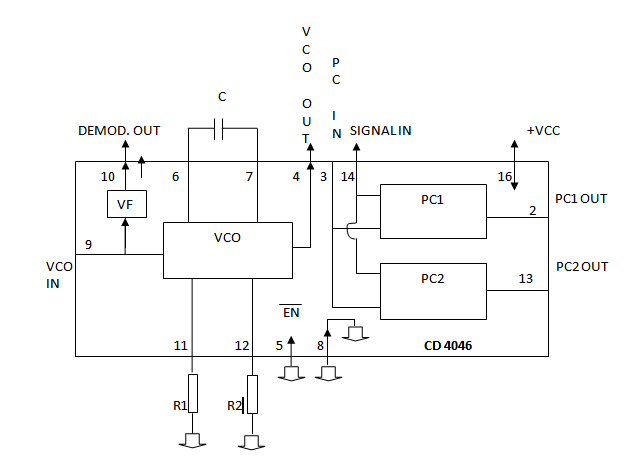
\includegraphics[width=\textwidth, height=8cm]{PLLBLOCK.png}
    \caption{Internal block Diagram of IC CD4046}
    \label{PLLBLOCK}
\end{figure}

\paragraph{}


It consists of a  linear voltage controlled oscilator (VCO) and two phase comparators. The two phase comparators have a common signal input terminal and a common comparator input terminals. The signal input terminal can be directly coupled for large input signal( upto $V_{CC}$) or capacitively coupled for small input signals (less than $\frac{	V_{CC}}{2}$). PC1 uses an XOR gate internally. Within the capture range, the output pulse width vary with the frequency difference between the signal input and the comparator input frequencies. Output amplitude is $V_{CC}$. PC1 gives a digital error signal tye pulse width of which depends on the phase difference between inputs. 

\paragraph{}Between the signal input frequency and the comparator input frequency, it may synchronise on to the signal frequencies that are close to VCo central frequency , $f_0$
or its harmonics.  PC2 is an edge triggered flip-flop circuit and its output is also proportional to the phase difference between two input frequencies. 

\paragraph{} The linear VCO produces an output frequency (pulses) whose amplitude depends on $V_{CC}$ only,  and the frequency depends on the the control voltage $V_C$ to be given to the VCO input terminal (VCOin) and resistors $R_1$ and $R_2$ and the capacitor C to be connected externally. This signal is obtained at VCOout terminal of the IC. The VCO sensitivity\footnote{oscillating voltage proportional to control voltage} is determined by $R_1$  and C and offset frequency\footnote{Frequency output at $V_C$=0} is determined by $R_1$  and C.

\paragraph{} A voltage follower is internally connected to the to the VCO input, the output of which is givena s demodulated output terminal of the IC. A pull down resistor (greater than 10 $k\Omega$) must be connected from the demodulated output terminal  to the ground. The output is taken across this resistor. For proper operation of the IC, the INHIBIT(/STROBE/ENABLE) terminal must be grounded.

The free running frequency $f_0$ is given by 
\begin{equation}
\label{f0}
f_{VCO}=\frac{0.16\ ( \frac{V_{CC}}{2} )}{R_1.C}+\frac{1}{R_2.C}
\end{equation}

